\documentclass{article}
\usepackage{amsmath,enumitem}
\usepackage{tikz}
\usepackage{tikz-uml}
\usepackage{geometry}
\geometry{margin=1in}
\title{Campus Drone Express - UI Design Assignment}
\author{StudentID\_Name}
\date{\today}

\begin{document}

\maketitle

\section{Interface Concept Design}
Below are the six interface classes along with their key elements.

\subsection{Order Placement Interface}
\begin{itemize}
    \item \textbf{Static Elements:} Header (Campus Drone Express title, navigation bar), instruction panels.
    \item \textbf{Dynamic Elements:} List of available books, order summary preview.
    \item \textbf{User Input Elements:} Text fields, dropdowns to select books and pickup times.
    \item \textbf{User Command Elements:} \texttt{Submit Order} button.
\end{itemize}

\subsection{Real-Time Drone Status Interface}
\begin{itemize}
    \item \textbf{Static Elements:} Map background, static legends for drone paths.
    \item \textbf{Dynamic Elements:} Live drone location indicator, battery meter, flight path overlay.
    \item \textbf{User Input Elements:} Toggle options (e.g., view satellite/terrain maps).
    \item \textbf{User Command Elements:} \texttt{Refresh Status} button.
\end{itemize}

\subsection{Emergency Control Interface}
\begin{itemize}
    \item \textbf{Static Elements:} Dashboard layout with emergency alert banner.
    \item \textbf{Dynamic Elements:} Alert messages, updated status when emergency commands are executed.
    \item \textbf{User Input Elements:} Optional text input for emergency details.
    \item \textbf{User Command Elements:} \texttt{Pause Drone} and \texttt{Return Drone} buttons.
\end{itemize}

\subsection{Route Maintenance Interface (Admin)}
\begin{itemize}
    \item \textbf{Static Elements:} Sidebar menu with list of routes, map overview.
    \item \textbf{Dynamic Elements:} Editable route lists and maps.
    \item \textbf{User Input Elements:} Forms for editing/adding routes.
    \item \textbf{User Command Elements:} \texttt{Save Route} and \texttt{Delete Route} controls.
\end{itemize}

\subsection{Firmware Update Interface (Admin)}
\begin{itemize}
    \item \textbf{Static Elements:} Current firmware version display, update instructions.
    \item \textbf{Dynamic Elements:} Update progress bar.
    \item \textbf{User Input Elements:} File upload control for new firmware packages.
    \item \textbf{User Command Elements:} \texttt{Initiate Update} button.
\end{itemize}

\subsection{Administrative Dashboard Interface}
\begin{itemize}
    \item \textbf{Static Elements:} Data panels for statistics, charts.
    \item \textbf{Dynamic Elements:} Real-time task analytics (e.g., number of orders, error logs).
    \item \textbf{User Input Elements:} Date range selectors, filter options.
    \item \textbf{User Command Elements:} \texttt{Generate Report} and \texttt{View Details} buttons.
\end{itemize}

\section{UML Class Diagram}
Using the mapping rules: \emph{window} $\rightarrow$ object class, \emph{interface element} $\rightarrow$ class attribute, and \emph{command} $\rightarrow$ class method, one possible UML class diagram is presented below.

\begin{center}
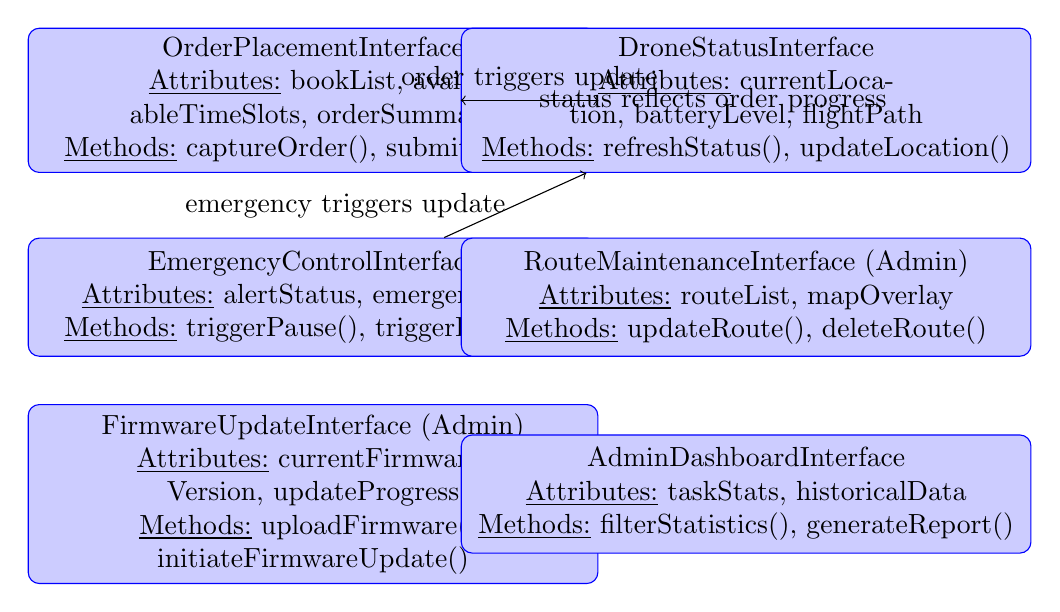
\begin{tikzpicture}[node distance=2.5cm]
    \tikzstyle{interface}=[rectangle,draw=blue,fill=blue!20,rounded corners, text width=7cm, align=center, minimum height=1.5cm]
    
    \node (order) [interface] {OrderPlacementInterface\\ \underline{Attributes:} bookList, availableTimeSlots, orderSummary\\ \underline{Methods:} captureOrder(), submitOrder()};
    
    \node (status) [interface, right of=order, xshift=3cm] {DroneStatusInterface\\ \underline{Attributes:} currentLocation, batteryLevel, flightPath\\ \underline{Methods:} refreshStatus(), updateLocation()};
    
    \node (emergency) [interface, below of=order] {EmergencyControlInterface\\ \underline{Attributes:} alertStatus, emergencyLog\\ \underline{Methods:} triggerPause(), triggerReturn()};
    
    \node (route) [interface, below of=status] {RouteMaintenanceInterface (Admin)\\ \underline{Attributes:} routeList, mapOverlay\\ \underline{Methods:} updateRoute(), deleteRoute()};
    
    \node (firmware) [interface, below of=emergency] {FirmwareUpdateInterface (Admin)\\ \underline{Attributes:} currentFirmwareVersion, updateProgress\\ \underline{Methods:} uploadFirmware(), initiateFirmwareUpdate()};
    
    \node (dashboard) [interface, below of=route] {AdminDashboardInterface\\ \underline{Attributes:} taskStats, historicalData\\ \underline{Methods:} filterStatistics(), generateReport()};
    
    % Arrows for associations and triggers
    \draw[->] (order) -- (status) node[midway, above] {order triggers update};
    \draw[->] (emergency) -- (status) node[midway, left] {emergency triggers update};
    \draw[->] (status) -- (order) node[midway, right] {status reflects order progress};
\end{tikzpicture}
\end{center}

\section{Interface Transition Sequence Diagram}
For the scenario where a student places an order and triggers an emergency drone return en route, the sequence diagram spans at least four interfaces:

\begin{enumerate}
    \item \textbf{Order Placement Interface:}
    \begin{itemize}
        \item The student inputs order details and presses \texttt{Submit Order}.
        \item Method \texttt{submitOrder()} is invoked.
    \end{itemize}
    
    \item \textbf{Drone Status Interface:}
    \begin{itemize}
        \item An order confirmation is displayed while the current drone status is shown.
        \item A status update message is sent to the drone control system.
    \end{itemize}
    
    \item \textbf{Emergency Control Interface:}
    \begin{itemize}
        \item The student, upon recognizing an emergency, presses the \texttt{Return Drone} button.
        \item Method \texttt{triggerReturn()} is called.
    \end{itemize}
    
    \item \textbf{Drone Control System:}
    \begin{itemize}
        \item Receives the emergency command.
        \item Initiates a corrective action, updating the Drone Status Interface accordingly.
    \end{itemize}
\end{enumerate}

\section{Design Principles Self-Evaluation}
The design meets key principles as described below:

\textbf{Intuitiveness:} \\
Each interface is organized logically, with clearly labeled input fields and buttons. Visual elements such as maps and progress bars facilitate a quick understanding of the system’s status.

\bigskip
\textbf{Ease of Use:} \\
The design minimizes the number of steps required for critical operations like order placement and emergency actions. Uniform layout and contextual tooltips help reduce user errors.

\bigskip
\textbf{Consistency:} \\
Uniform design elements (e.g., similar button placements and color coding for alerts) ensure a coherent experience across different interfaces.

\bigskip
\textbf{Fault Tolerance:} \\
The system incorporates features such as confirmation dialogs, real-time status updates, and immediate emergency overrides to handle errors and issues gracefully.

\bigskip
\textbf{Human-Centered Design:} \\
The interface design accommodates a wide range of users by offering simplified modes for novices and detailed functionalities for advanced users. Two improvements identified are enhancing accessibility for users with disabilities and optimizing the design for mobile responsiveness, particularly for image-rich content.

\end{document}
